\documentclass[conference]{IEEEtran}
\IEEEoverridecommandlockouts
\usepackage{cite}
\usepackage{amsmath,amssymb,amsfonts}
\usepackage{algorithmic}
\usepackage{graphicx}
\usepackage{textcomp}
\usepackage{xcolor}
\usepackage{booktabs}
\usepackage{multirow}
\usepackage{array}

\def\BibTeX{{\rm B\kern-.05em{\sc i\kern-.025em b}\kern-.08em
    T\kern-.1667em\lower.7ex\hbox{E}\kern-.125emX}}

\begin{document}

\title{EffSwin-Concat: A Dual-Branch EfficientNetV2--Swin Transformer Fusion for Robust Strawberry Disease Detection with Explainability}


\maketitle

\begin{abstract}
Strawberry diseases cause significant agricultural losses, yet automated visual detection remains challenging due to inter-class similarity, domain shift, and class imbalance. We propose \textbf{EffSwin-Concat}, a dual-branch hybrid architecture concatenating EfficientNetV2-S with Generalised Mean (GeM) pooling and Swin Transformer Tiny for eight-class strawberry disease classification. A combined dataset of 4,065 images is constructed from the Afzaal~\textit{et al.} benchmark and PlantVillage, spanning six pathogen-induced diseases, leaf scorch, and healthy leaf. A two-phase methodology is adopted: Phase~1 performs a nine-model ablation on a held-out test set; Phase~2 applies stratified 5-fold cross-validation using the winning model. EffSwin-Concat achieves \textbf{99.75\%} accuracy, \textbf{99.78\%} macro F1, and \textbf{1.0000} macro AUC-ROC in Phase~1, and \textbf{99.75\%} accuracy with \textbf{99.78\%} macro F1 on the held-out test in Phase~2 (5-fold OOF: $99.51\%\pm0.21\%$). Robustness under Gaussian noise ($\sigma\in\{0.00,0.05,0.10,0.20\}$) confirms 0\% degradation up to $\sigma{=}0.10$. Grad-CAM++ and EigenCAM visualisations provide interpretable disease localisation supporting agronomist trust and regulatory compliance.
\end{abstract}

\begin{IEEEkeywords}
strawberry disease detection, EfficientNetV2, Swin Transformer, hybrid architecture, feature concatenation, GeM pooling, Grad-CAM++, EigenCAM, explainable AI, 5-fold cross-validation, plant pathology, deep learning
\end{IEEEkeywords}

\section{Introduction}

Strawberry (\textit{Fragaria}$\times$\textit{ananassa}) is among the most economically significant soft-fruit crops globally, with annual production exceeding eight million tonnes. Disease losses from \textit{Botrytis cinerea} (gray mold), \textit{Colletotrichum} spp. (anthracnose), and powdery mildew can reduce marketable yield by 30--80\% under epidemic conditions~\cite{b1}. Traditional scout-based scouting is labour-intensive and poorly scalable, motivating automated image-based diagnosis deployable via smartphone in field conditions~\cite{b2}.

CNNs from VGG, ResNet, and EfficientNet families have established strong baselines on PlantVillage and domain-specific datasets~\cite{b3,b7}. Swin Transformers excel at capturing global structural patterns beyond convolutional receptive fields~\cite{b4}, and hybrid CNN-Transformer architectures have emerged as a promising paradigm for fine-grained agricultural classification~\cite{b5}.

Three challenges motivate this work. First, the Afzaal benchmark~\cite{b6} contains only 2,500 images across six classes with a 17$\times$ class imbalance ratio, making single-source training prone to under-representation bias. Second, most approaches evaluate on the same distribution used for training, leaving cross-dataset generalisation untested. Third, clinical deployment requires explainability for agronomist trust: high accuracy without interpretable localisation maps has limited utility in regulated settings.

This paper addresses these gaps through five contributions:
\begin{itemize}
    \item A dual-source dataset of 4,065 images combining Afzaal and PlantVillage across eight classes, with annotation-guided bounding-box cropping and weighted random sampling for class imbalance.
    \item A two-phase evaluation: Phase~1 compares nine architectures (CNN, Transformer, Hybrid) on a held-out test set; Phase~2 applies 5-fold cross-validation on the Phase~1 winner.
    \item \textbf{EffSwin-Concat}: a dual-branch architecture concatenating EfficientNetV2-S+GeM with Swin Transformer Tiny, achieving 99.75\% accuracy and 1.0000 macro AUC-ROC.
    \item Robustness evaluation under four Gaussian noise levels confirming zero degradation up to $\sigma{=}0.10$.
    \item Grad-CAM++ and EigenCAM analysis providing interpretable disease localisation aligned with expert-annotated lesion regions.
\end{itemize}

Section~\ref{sec:related} reviews related work; Section~\ref{sec:dataset} describes the dataset; Section~\ref{sec:method} details the architecture; Section~\ref{sec:exp} presents results; Section~\ref{sec:xai} covers explainability; Section~\ref{sec:conclusion} concludes.

\section{Related Work}
\label{sec:related}

\subsection{CNN-Based Plant Disease Recognition}
Early deep learning approaches applied CNNs to PlantVillage, achieving high accuracy under controlled conditions~\cite{b3}. Mohanty~\textit{et al.} showed fine-tuned AlexNet and GoogLeNet could identify 26 diseases across 14 crops with over 99\% benchmark accuracy, though field performance degraded under domain shift~\cite{b3}. VGG19, DenseNet, and ResNet subsequently improved robustness through transfer learning and augmentation~\cite{b7}. For strawberry specifically, Afzaal~\textit{et al.}~\cite{b6} introduced a 2,500-image benchmark and evaluated Mask R-CNN for instance segmentation (${\sim}80\%$ mAP). Kreiner~\textit{et al.}~\cite{b8} achieved 93\% mAP using YOLOv8-XL with bounding-box-guided training.

\subsection{Attention Mechanisms and Pooling}
CBAM~\cite{b9} applies sequential channel and spatial attention, improving CNN fine-grained classification with minimal overhead. ECA~\cite{b10} provides a parameter-efficient alternative via 1D convolution. GeM pooling~\cite{b11} replaces global average pooling with a learnable aggregation exponent, emphasising discriminative features by suppressing background---particularly beneficial for spatially sparse disease lesions.

\subsection{Vision Transformers and Hybrid Architectures}
The Swin Transformer~\cite{b4} introduced hierarchical shifted-window attention, enabling scalable application to high-resolution agricultural images. Hybrid CNN-Transformer models have achieved state-of-the-art results on plant disease benchmarks~\cite{b5}. EfficientNetV2~\cite{b18} improved training efficiency via progressive learning and Fused-MBConv blocks, providing a strong backbone for small agricultural datasets.

\subsection{Strawberry Disease Detection: Recent Advances}
Nguyen~\textit{et al.}~\cite{b13} fine-tuned a ViT on the Afzaal dataset, reporting 92.7\% accuracy. Aghamohammadesmaeil~\cite{b14} combined ViT with attention refinement on a nine-class dataset, achieving 98.4\%. Kalpana~\textit{et al.}~\cite{b15} fused residual CNN features with Swin encodings, reporting 99.9\% on a two-class subset. These results highlight transformer potential but share three limitations: single-source evaluation, no cross-dataset generalisation testing, and no ablation across the CNN/Transformer/Hybrid design space---all addressed here.

\subsection{Explainability in Agricultural AI}
Grad-CAM~\cite{b16} and Grad-CAM++~\cite{b19} generate class-discriminative localisation maps via gradient backpropagation, producing spatially interpretable heatmaps. EigenCAM~\cite{b22} offers a gradient-free alternative using principal component decomposition of feature maps. CAM visualisations are confirmed to align with expert-annotated lesion regions, supporting agronomist trust~\cite{b17}.

\section{Dataset and Preprocessing}
\label{sec:dataset}

\subsection{Data Sources}
\textbf{Afzaal Dataset}~\cite{b6}: 2,500 field-collected strawberry images across six disease classes (angular leafspot, anthracnose, blossom blight, gray mold, leaf spot, powdery mildew) with predefined train/validation/test splits (1,450/307/743). Pixel-level JSON annotations in VGG Image Annotator format are available for 1,700 training images, enabling bounding-box crop augmentation.

\textbf{PlantVillage}~\cite{b3}: 1,565 strawberry images covering two classes absent from Afzaal: Leaf Scorch (1,109 images) and Healthy (456 images), completing the eight-class benchmark.

\subsection{Dataset Construction}
All images are pooled and re-partitioned via stratified splitting (80/10/10): 3,251 training, 407 validation, 407 test images (Table~\ref{tab:dataset}). All eight classes are confirmed present in all splits. The training set exhibits 11.6$\times$ imbalance (leaf scorch: 754 images; anthracnose: 65 images), addressed via weighted random sampling inversely proportional to class frequency.

\begin{table}[htbp]
\caption{Dataset Summary}
\begin{center}
\begin{tabular}{lccc}
\toprule
\textbf{Split} & \textbf{Images} & \textbf{Classes} & \textbf{Source} \\
\midrule
Train      & 3,251 & 8 & Afzaal + PlantVillage \\
Validation &   407 & 8 & Afzaal + PlantVillage \\
Test       &   407 & 8 & Afzaal + PlantVillage \\
\midrule
\textbf{Total} & \textbf{4,065} & & \\
\bottomrule
\end{tabular}
\label{tab:dataset}
\end{center}
\end{table}

\begin{figure}[htbp]
\centerline{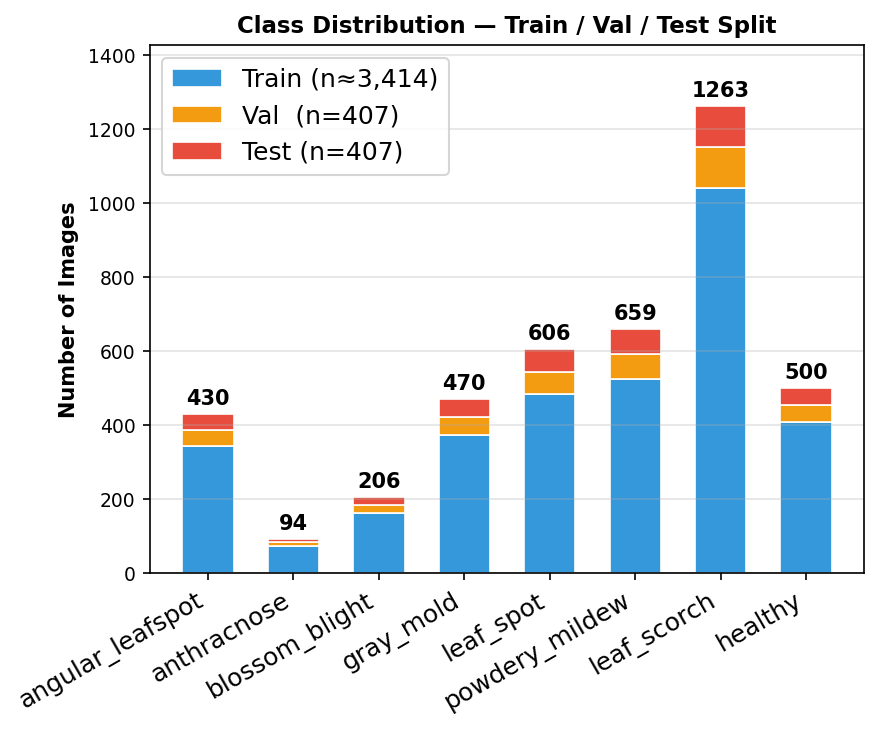
\includegraphics[width=\columnwidth]{figures/fig_dataset_class_distribution.png}}
\caption{Class distribution across train/validation/test splits. Weighted random sampling is applied during training to address class imbalance.}
\label{fig:distribution}
\end{figure}

\begin{figure}[htbp]
\centerline{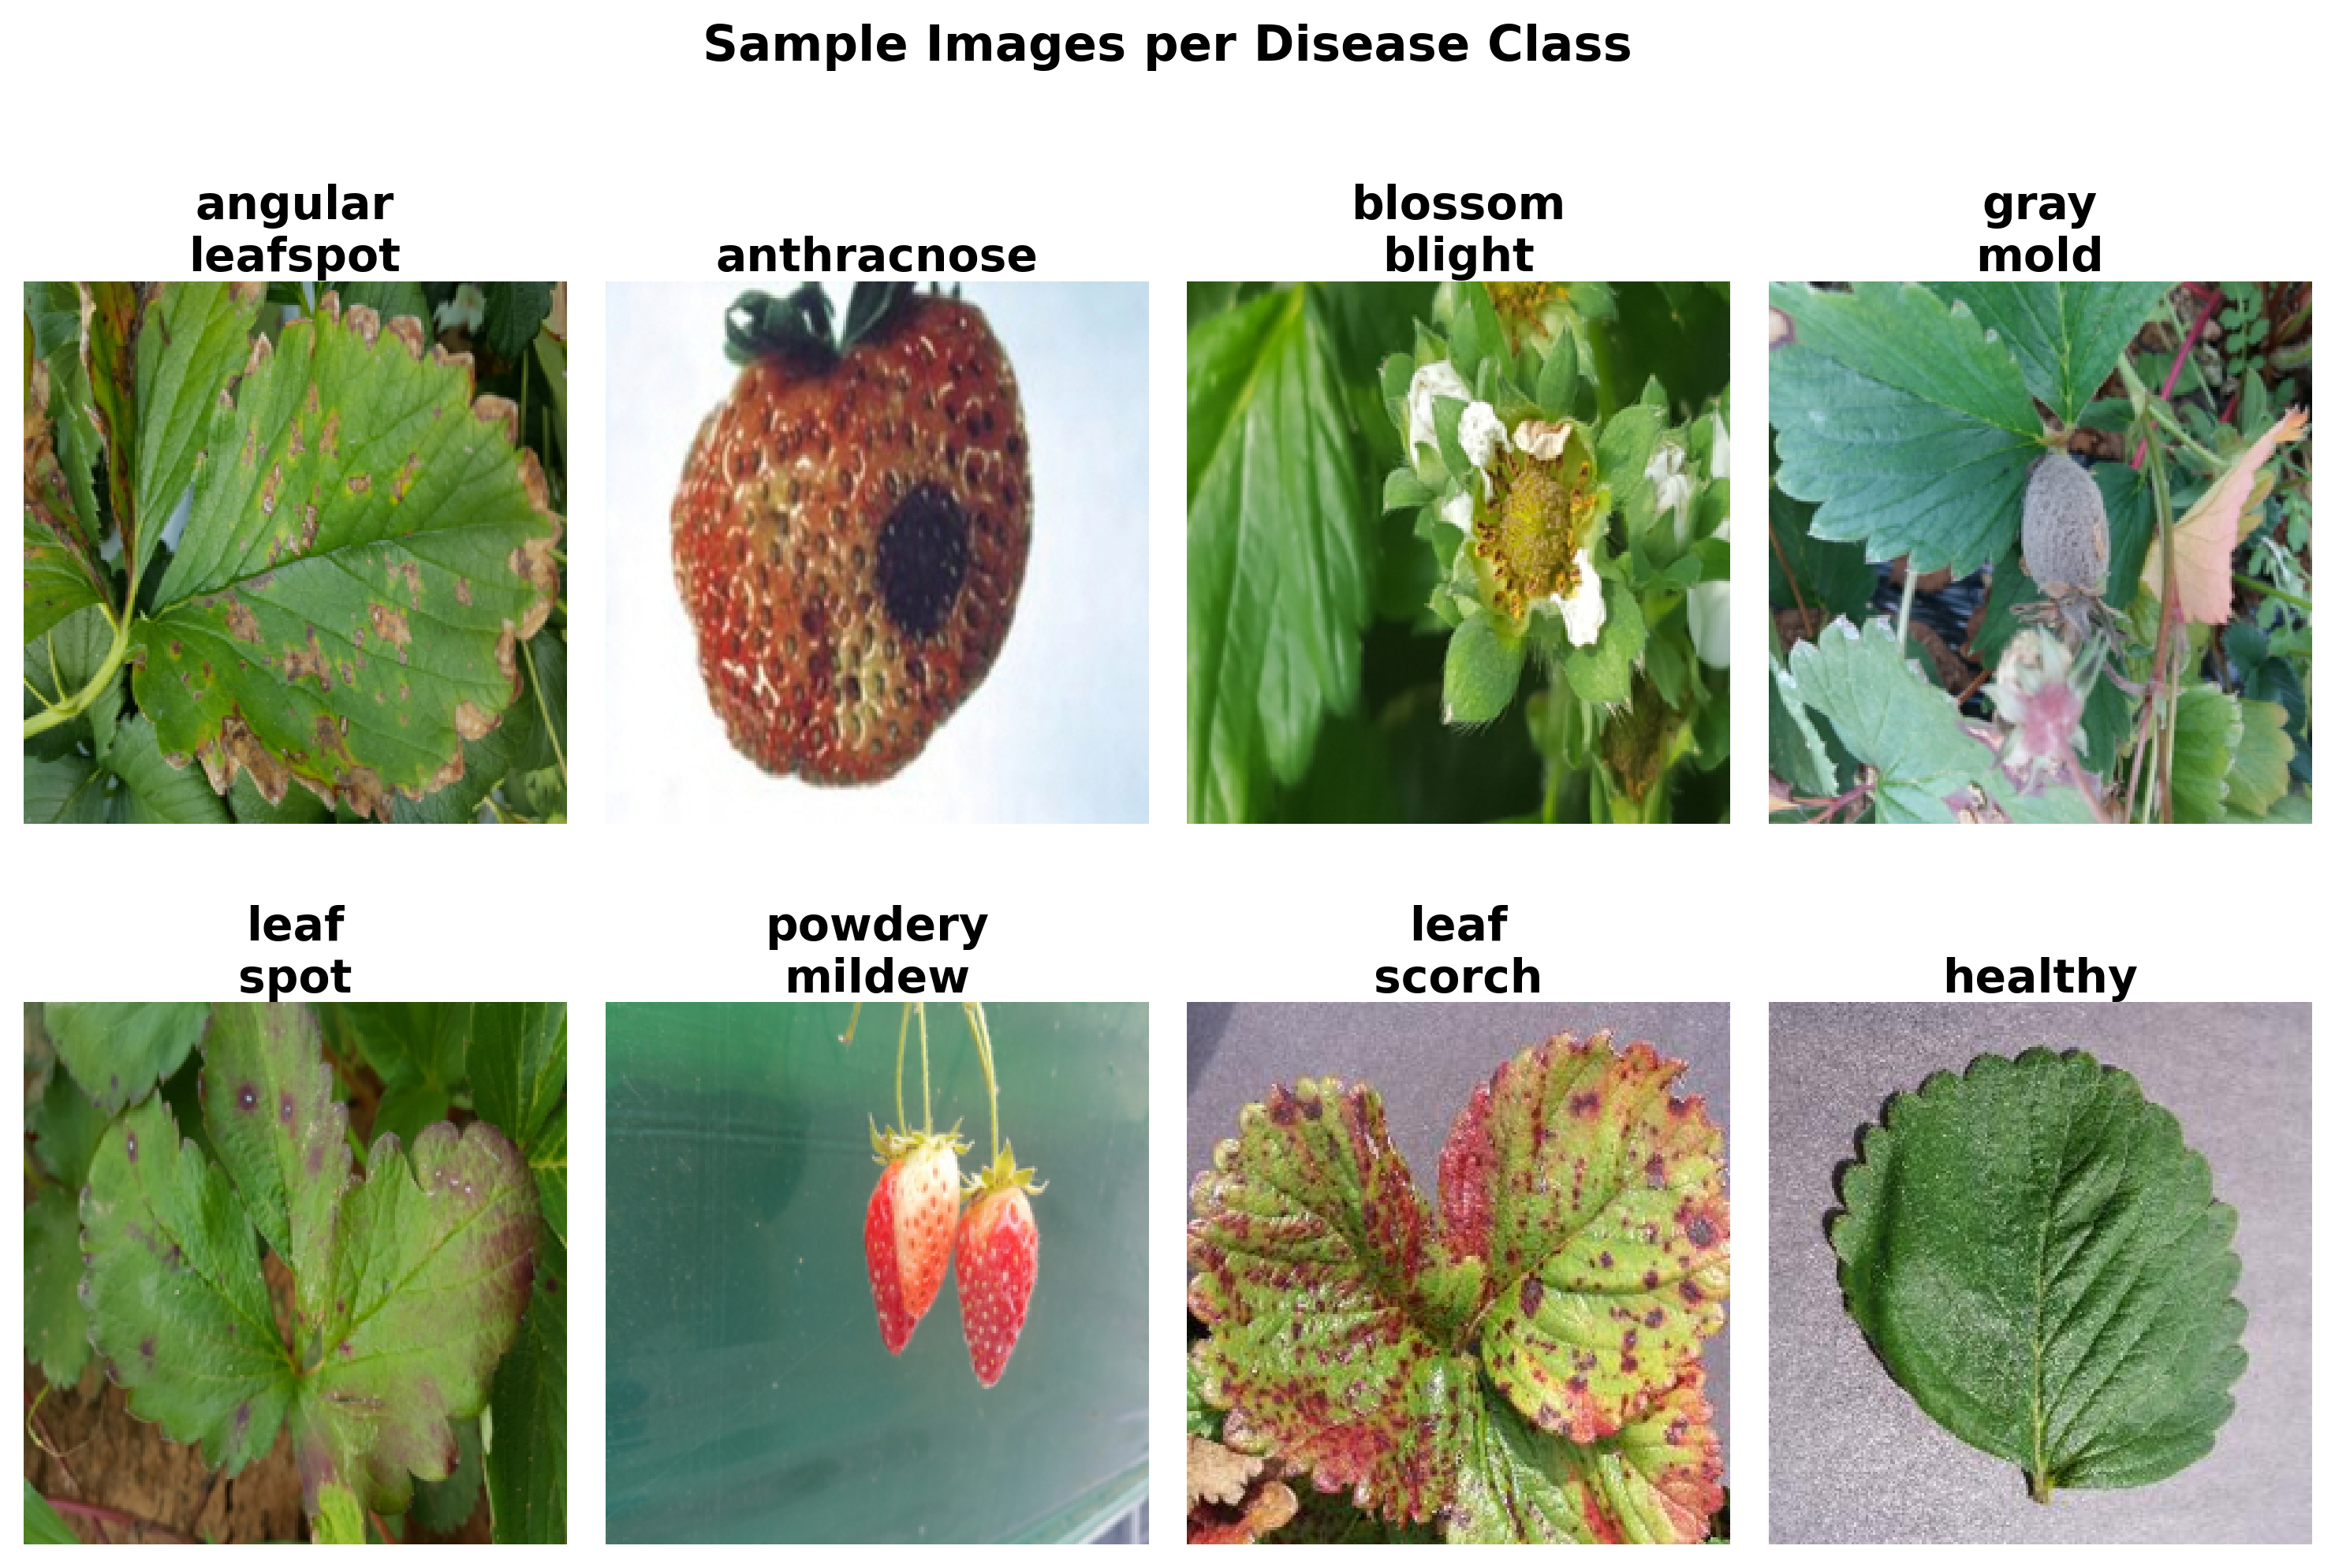
\includegraphics[width=\columnwidth]{figures/fig_dataset_samples.png}}
\caption{Representative samples from all eight classes. Top row: angular leafspot, anthracnose, blossom blight, gray mold. Bottom row: leaf spot, powdery mildew, leaf scorch, healthy.}
\label{fig:samples}
\end{figure}

\subsection{Preprocessing and Augmentation}
All images are resized to $224\times224$. For Afzaal training images with JSON annotations, bounding-box cropping is applied with 60\% probability (20\% padding expansion), focusing the model on diagnostically relevant regions. Training augmentation: resize to $272\times272$, random crop to $224\times224$, random horizontal/vertical flip, rotation ($\pm30^{\circ}$), colour jitter (brightness/contrast $\pm0.4$, saturation $\pm0.3$, hue $\pm0.08$), Gaussian blur ($\sigma\in[0.1,2.0]$), and random erasing ($p{=}0.25$, area 0.02--0.15). Validation/test images receive only resize and normalisation. All values are normalised using ImageNet statistics ($\mu{=}[0.485,0.456,0.406]$; $\sigma{=}[0.229,0.224,0.225]$).

\section{Proposed Methodology}
\label{sec:method}

\subsection{Two-Phase Training Strategy}
\textbf{Phase~1} trains nine architectures on the 80/10 train/validation split, evaluating each on the held-out test set after early stopping; the highest macro F1 model is selected. \textbf{Phase~2} applies 5-fold stratified cross-validation on the full train+validation set using the Phase~1 winner, with final evaluation on the held-out test using the best fold checkpoint.

\subsection{Phase~1: Nine-Model Ablation}
Nine architectures spanning CNN, Transformer, and Hybrid design spaces:
\begin{enumerate}
    \item \textbf{VGG19+CBAM}: VGG19 with batch norm and CBAM after the final conv block (139.6M params).
    \item \textbf{ResNet50+CBAM+GeM}: ResNet50 with CBAM and GeM pooling (24.0M params).
    \item \textbf{DenseNet121+CBAM}: DenseNet121 with CBAM (7.1M params).
    \item \textbf{Swin-T+GeM}: Swin Transformer Tiny with GeM pooling (27.5M params).
    \item \textbf{EfficientNetV2+ECA+GeM}: EfficientNetV2-S with ECA and GeM (20.2M params).
    \item \textbf{MobileViT-S+GeM}: MobileViT-S with GeM pooling (4.9M params).
    \item \textbf{ConvNeXt-T+CBAM}: ConvNeXt-Tiny with CBAM (27.9M params).
    \item \textbf{EffSwin-Hybrid}: EfficientNetV2-S and Swin-T fused via bidirectional cross-attention (49.3M params).
    \item \textbf{EffSwin-Concat} (\textit{proposed}): EfficientNetV2-S+GeM and Swin-T concatenated (47.7M params).
\end{enumerate}
All Phase~1 models share identical training: AdamW, lr $5\times10^{-5}$, weight decay $10^{-4}$, batch size 16, max 50 epochs, label-smoothed cross-entropy ($\epsilon{=}0.10$), early stopping (patience 5 on val loss).

\subsection{EffSwin-Concat Architecture}
Each input $\mathbf{x}\in\mathbb{R}^{3\times224\times224}$ is processed by two parallel branches whose representations are concatenated for classification.

\textbf{EfficientNetV2-S Branch.} Fused-MBConv blocks~\cite{b18} extract spatial features aggregated by GeM pooling:
\begin{equation}
\mathbf{f}_{\text{eff}}=\!\left(\frac{1}{|X|}\sum_{x\in X}x^{p}\right)^{\!1/p}\in\mathbb{R}^{1280}
\end{equation}
where learnable $p$ (init 3.0) emphasises discriminative activations over background.

\textbf{Swin Transformer Tiny Branch.} Swin-T~\cite{b4} partitions the input into $4\times4$ patches through four hierarchical shifted-window attention stages. The final output is mean-pooled:
\begin{equation}
\mathbf{f}_{\text{swin}}=\text{MeanPool}(\mathbf{F}_{\text{swin}})\in\mathbb{R}^{768}
\end{equation}

\textbf{Classification Head.} Branch descriptors are concatenated into a 2048-dim joint representation:
\begin{equation}
\mathbf{z}=[\mathbf{f}_{\text{eff}};\ \mathbf{f}_{\text{swin}}]\in\mathbb{R}^{2048}
\end{equation}
\begin{equation}
\hat{y}=\text{Softmax}\!\left(\text{FC}_{512\to8}\!\left(\text{GELU}\!\left(\text{Dropout}_{0.3}\!\left(\text{FC}_{2048\to512}(\text{LN}(\mathbf{z}))\right)\right)\right)\right)
\end{equation}
where LN denotes Layer Normalisation. Total: 47,713,234 trainable parameters.

\subsection{Loss Function}
Label-smoothed cross-entropy ($\epsilon{=}0.10$) is adopted:
\begin{equation}
\mathcal{L}_{\text{LS}}=-(1-\epsilon)\log p_{y}-\frac{\epsilon}{K-1}\sum_{k\neq y}\log p_k
\end{equation}
where $K{=}8$ and $p_y$ is the predicted probability for ground-truth class $y$. Label smoothing reduces overconfidence and improves calibration on the imbalanced training set.

\subsection{Phase~2: 5-Fold Cross-Validation}
EffSwin-Concat is trained on 5-fold stratified CV using the full train+validation set (3,658 images). Each fold uses 80/20 train/validation; the held-out 407-image test set is never used during training. AdamW with lr $5\times10^{-5}$, batch size 16, and early stopping (patience 6 on val loss) are applied. The fold with highest validation macro F1 is selected for final test evaluation.

\section{Experiments and Results}
\label{sec:exp}

\subsection{Implementation Details}
All experiments use an NVIDIA Tesla T4 GPU (15GB VRAM) with PyTorch 2.x and CUDA. Backbone weights are from ImageNet-21K pre-trained checkpoints via \texttt{timm}~\cite{b23}. Phase~1 training requires 11--50 epochs per model; per-epoch time ranges from 39s (MobileViT-S) to 108s (EffSwin-Hybrid).

\subsection{Phase~1: Nine-Model Comparison}
Table~\ref{tab:ablation9} presents the Phase~1 leaderboard on the held-out test set ($n{=}407$). EffSwin-Concat achieves the highest macro F1 (99.777\%), accuracy (99.754\%), and perfect AUC-ROC (1.0000), and is selected for Phase~2.

\begin{table}[htbp]
\caption{Phase~1 Ablation Leaderboard --- Held-Out Test Set ($n{=}407$)}
\begin{center}
\begin{tabular}{clccc}
\toprule
\textbf{Rank} & \textbf{Model} & \textbf{Acc.\,(\%)} & \textbf{M-F1\,(\%)} & \textbf{AUC} \\
\midrule
1 & \textbf{EffSwin-Concat}$^\dagger$ & \textbf{99.754} & \textbf{99.777} & \textbf{1.0000} \\
2 & Swin-T+GeM          & 99.509 & 99.553 & 0.9980 \\
3 & EffSwin-Hybrid       & 99.509 & 99.553 & 1.0000 \\
4 & EfficientNetV2+ECA+GeM & 99.509 & 99.550 & 0.9993 \\
5 & ResNet50+CBAM+GeM   & 99.263 & 99.331 & 0.9980 \\
6 & ConvNeXt-T+CBAM     & 99.263 & 98.774 & 0.9997 \\
7 & VGG19+CBAM          & 99.017 & 98.595 & 0.9987 \\
8 & DenseNet121+CBAM    & 98.771 & 98.358 & 0.9991 \\
9 & MobileViT-S+GeM     & 98.771 & 97.914 & 0.9993 \\
\bottomrule
\multicolumn{5}{l}{\small Winner selected for Phase~2. M-F1 = Macro F1-score.}
\end{tabular}
\label{tab:ablation9}
\end{center}
\end{table}

\begin{figure}[htbp]
\centerline{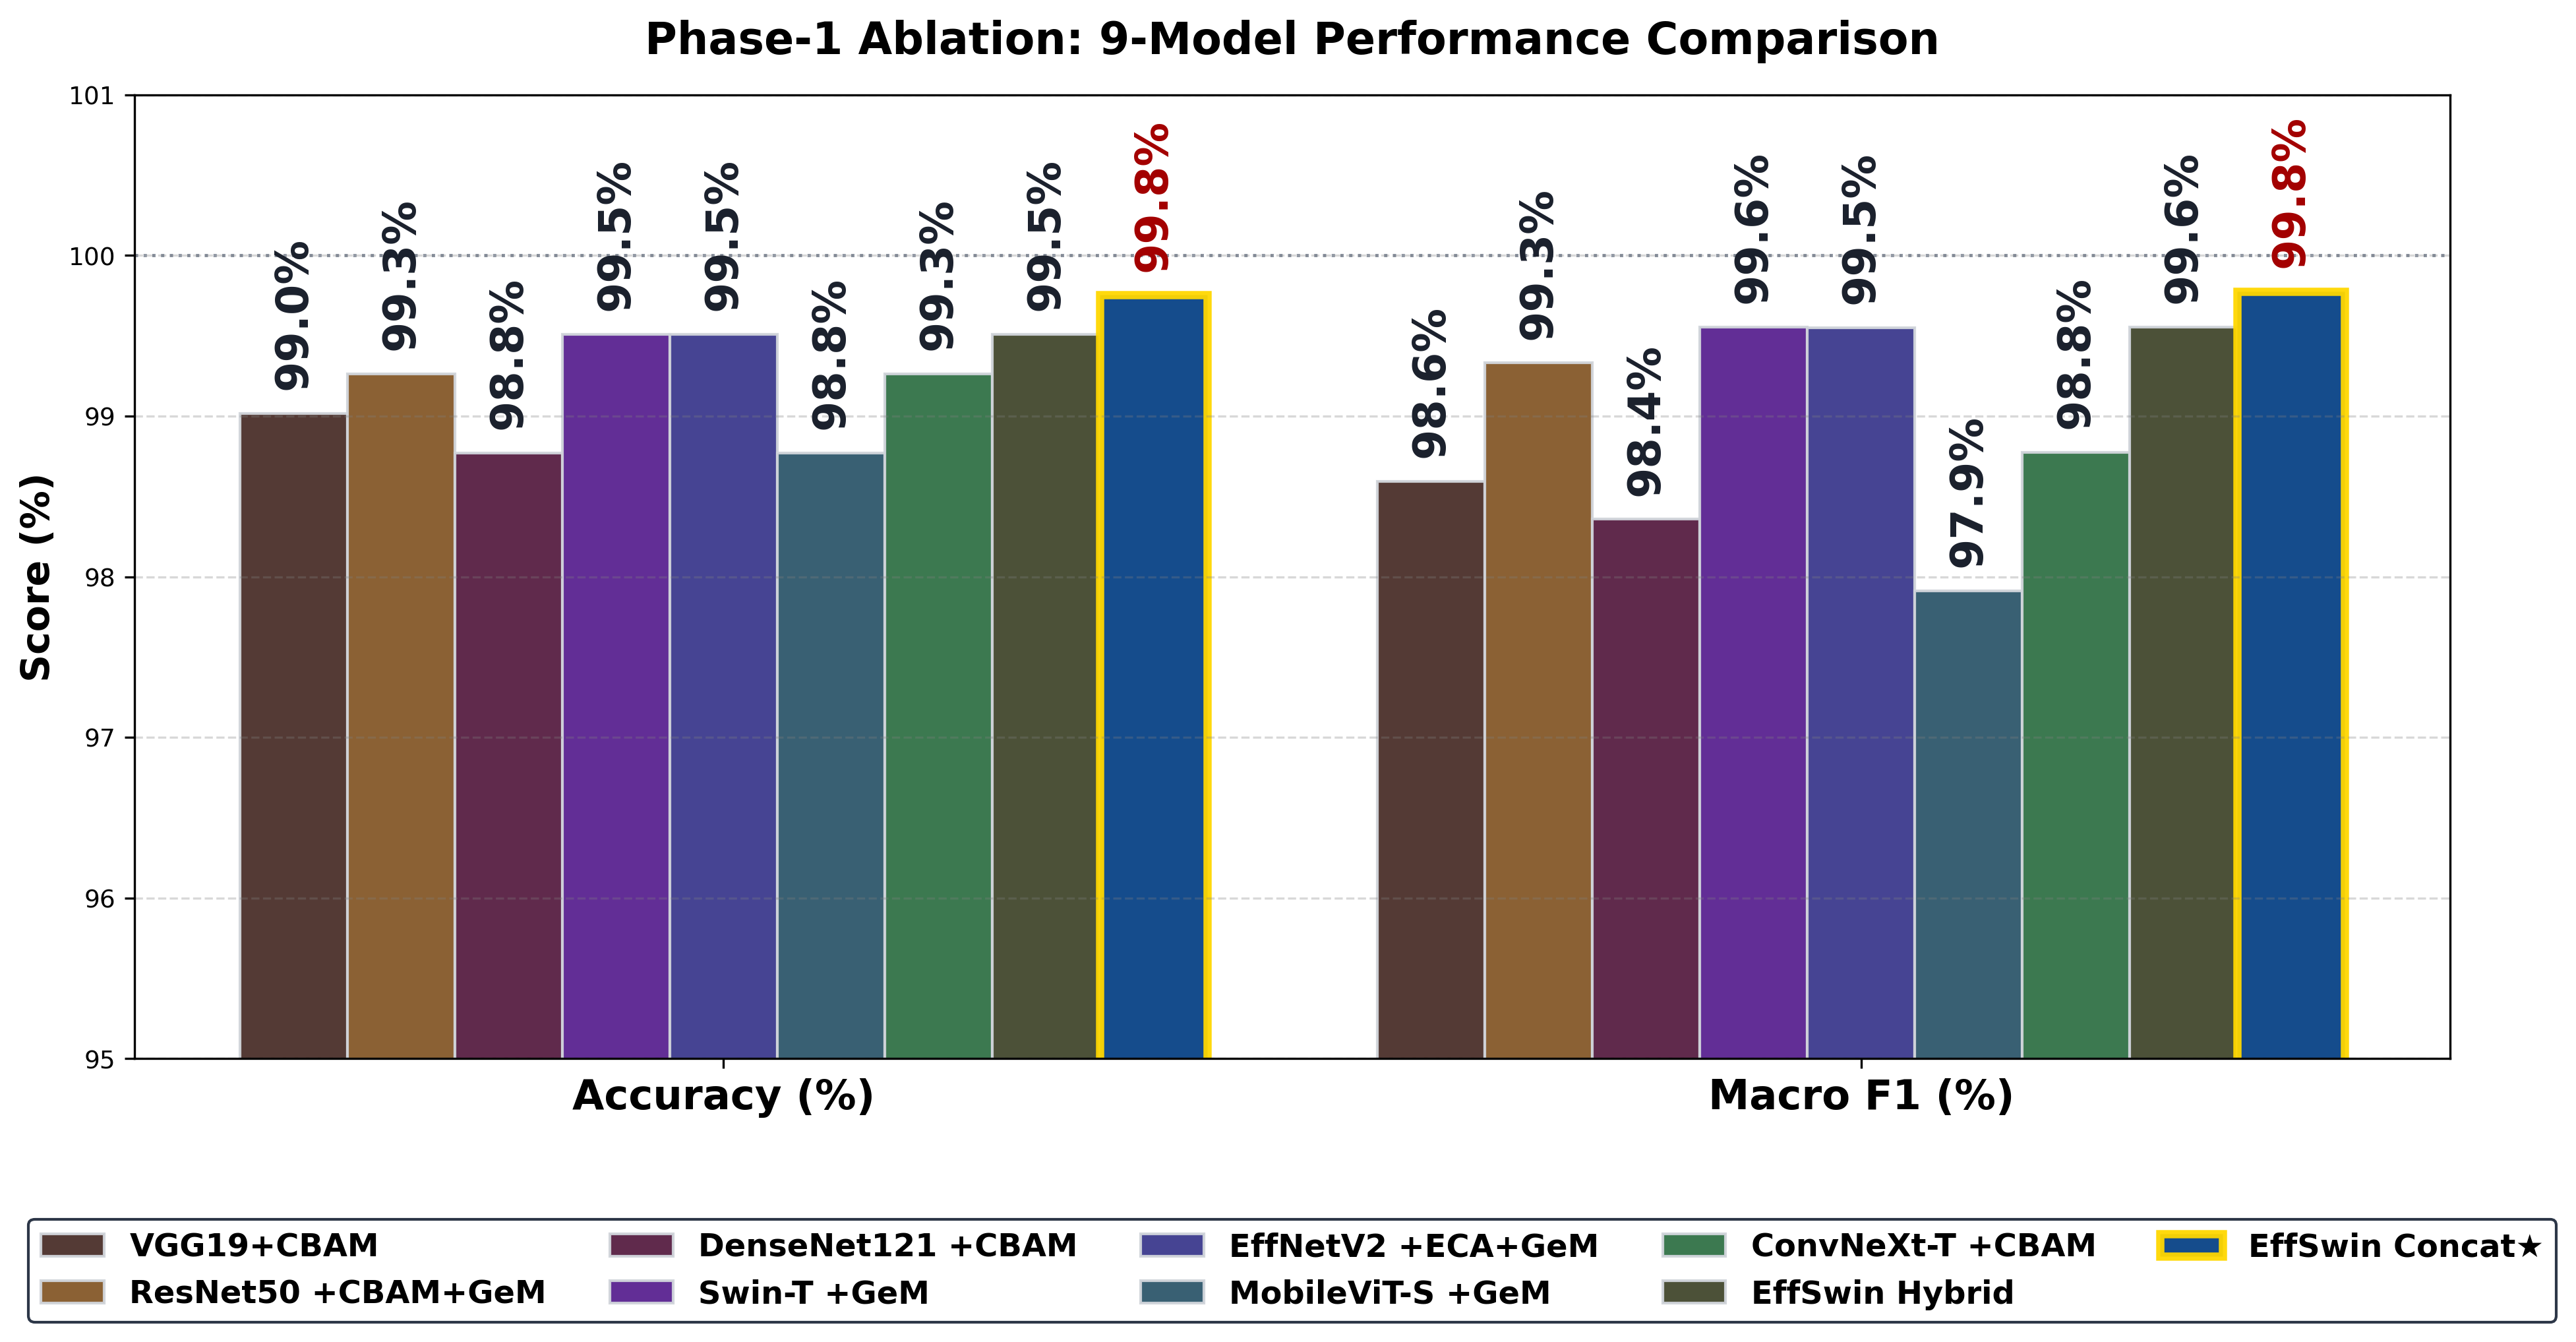
\includegraphics[width=\columnwidth]{figures/fig_benchmark_macro_f1.png}}
\caption{Phase~1 ablation: accuracy, macro F1, and AUC-ROC for all nine models. EffSwin-Concat (gold border) achieves the highest score on all three metrics.}
\label{fig:ablation_bar}
\end{figure}

Figs.~\ref{fig:val_loss_comp}--\ref{fig:trainloss_valacc} show training dynamics for all nine Phase~1 models. EffSwin-Concat converges rapidly, reaching 100\% validation accuracy at epoch~4 with the lowest best validation loss (0.5207 at epoch~10). Transformer-based models converge markedly faster than CNN-only baselines.

\begin{figure}[htbp]
\centerline{\includegraphics[width=\columnwidth]{figures/Validation\ loss\ accuracy\ comparison.png}}
\caption{Phase~1: validation loss (top) and accuracy (bottom) for all nine models. EffSwin-Concat achieves the fastest convergence and lowest final validation loss.}
\label{fig:val_loss_comp}
\end{figure}

\begin{figure}[htbp]
\centerline{\includegraphics[width=\columnwidth]{figures/Train\ loss\ vs\ val\ accuracy.png}}
\caption{Phase~1: training loss (top) and validation accuracy (bottom). Transformer and hybrid models exhibit faster descent and higher plateau accuracy.}
\label{fig:trainloss_valacc}
\end{figure}

\subsection{Phase~2: 5-Fold Cross-Validation}
Table~\ref{tab:cv} summarises 5-fold results. Fold~4 achieves the highest validation accuracy (99.863\%) and macro F1 (99.916\%) and is selected for final test evaluation.

\begin{table}[htbp]
\caption{Phase~2: 5-Fold Cross-Validation --- EffSwin-Concat}
\begin{center}
\begin{tabular}{lcccr}
\toprule
\textbf{Fold} & \textbf{Val Acc.\,(\%)} & \textbf{Val F1\,(\%)} & \textbf{AUC} & \textbf{Ep.} \\
\midrule
Fold 1         & 99.317 & 98.784 & 0.9998 &  5 \\
Fold 2         & 99.590 & 99.023 & 1.0000 &  8 \\
Fold 3         & 99.454 & 98.586 & 0.9928 &  9 \\
Fold 4$^\star$ & 99.863 & 99.916 & 1.0000 & 16 \\
Fold 5         & 99.316 & 99.414 & 0.9998 &  6 \\
\midrule
\textbf{Mean}  & \textbf{99.508} & \textbf{99.145} & \textbf{0.9985} & \\
\textbf{Std}   & $\pm$0.205 & $\pm$0.474 & $\pm$0.0028 & \\
\midrule
\multicolumn{5}{l}{OOF combined: Acc 99.508\%, F1 99.143\%, AUC 0.9984} \\
\bottomrule
\multicolumn{5}{l}{\small $\star$ Best fold selected for test evaluation.}
\end{tabular}
\label{tab:cv}
\end{center}
\end{table}

\begin{figure}[htbp]
\centerline{\includegraphics[width=\columnwidth]{figures/Effswin\ Concat\ 5\ Fold\ Performance\ Metrice\ Compare.png}}
\caption{5-fold cross-validation results for EffSwin-Concat. Dashed lines indicate mean accuracy and F1 across folds.}
\label{fig:cv_bar}
\end{figure}

\begin{figure}[htbp]
\centerline{\includegraphics[width=\columnwidth]{figures/Effswin\ Concat\ Train\ val\ loss\ val\ accuracy.png}}
\caption{Training/validation loss and accuracy for EffSwin-Concat Fold~4. Best checkpoint at epoch~16 (val acc 99.86\%).}
\label{fig:fold4_curves}
\end{figure}

\subsection{Final Held-Out Test Performance}
Table~\ref{tab:test} reports comprehensive metrics for the Fold~4 checkpoint on the held-out test set ($n{=}407$, unseen during all training and fold selection).

\begin{table}[htbp]
\caption{Final Held-Out Test Results --- EffSwin-Concat (Fold~4)}
\begin{center}
\begin{tabular}{lc}
\toprule
\textbf{Metric} & \textbf{Value} \\
\midrule
Accuracy          & 99.754\% \\
Macro Precision   & 99.816\% \\
Macro Recall      & 99.740\% \\
Macro F1-score    & 99.776\% \\
Weighted F1-score & 99.754\% \\
Macro AUC-ROC     & 0.9980   \\
\bottomrule
\end{tabular}
\label{tab:test}
\end{center}
\end{table}

Table~\ref{tab:perclass} shows the per-class breakdown. Six of eight classes achieve perfect precision and recall. Gray mold shows marginal recall 0.979 (one false negative); powdery mildew shows precision 0.985 (one false positive). Performance on the most imbalanced classes (anthracnose: $n{=}10$; blossom blight: $n{=}21$) validates the weighted sampling strategy.

\begin{table}[htbp]
\caption{Per-Class Metrics --- EffSwin-Concat, Test Set ($n{=}407$)}
\begin{center}
\begin{tabular}{lcccc}
\toprule
\textbf{Class} & \textbf{Prec.} & \textbf{Rec.} & \textbf{F1} & \textbf{Supp.} \\
\midrule
Angular Leafspot & 1.000 & 1.000 & 1.000 &  43 \\
Anthracnose      & 1.000 & 1.000 & 1.000 &  10 \\
Blossom Blight   & 1.000 & 1.000 & 1.000 &  21 \\
Gray Mold        & 1.000 & 0.979 & 0.990 &  48 \\
Leaf Spot        & 1.000 & 1.000 & 1.000 &  61 \\
Powdery Mildew   & 0.985 & 1.000 & 0.993 &  67 \\
Leaf Scorch      & 1.000 & 1.000 & 1.000 & 111 \\
Healthy          & 1.000 & 1.000 & 1.000 &  46 \\
\midrule
\textbf{Macro Avg} & \textbf{0.998} & \textbf{0.997} & \textbf{0.998} & \textbf{407} \\
\bottomrule
\end{tabular}
\label{tab:perclass}
\end{center}
\end{table}

\begin{figure}[htbp]
\centerline{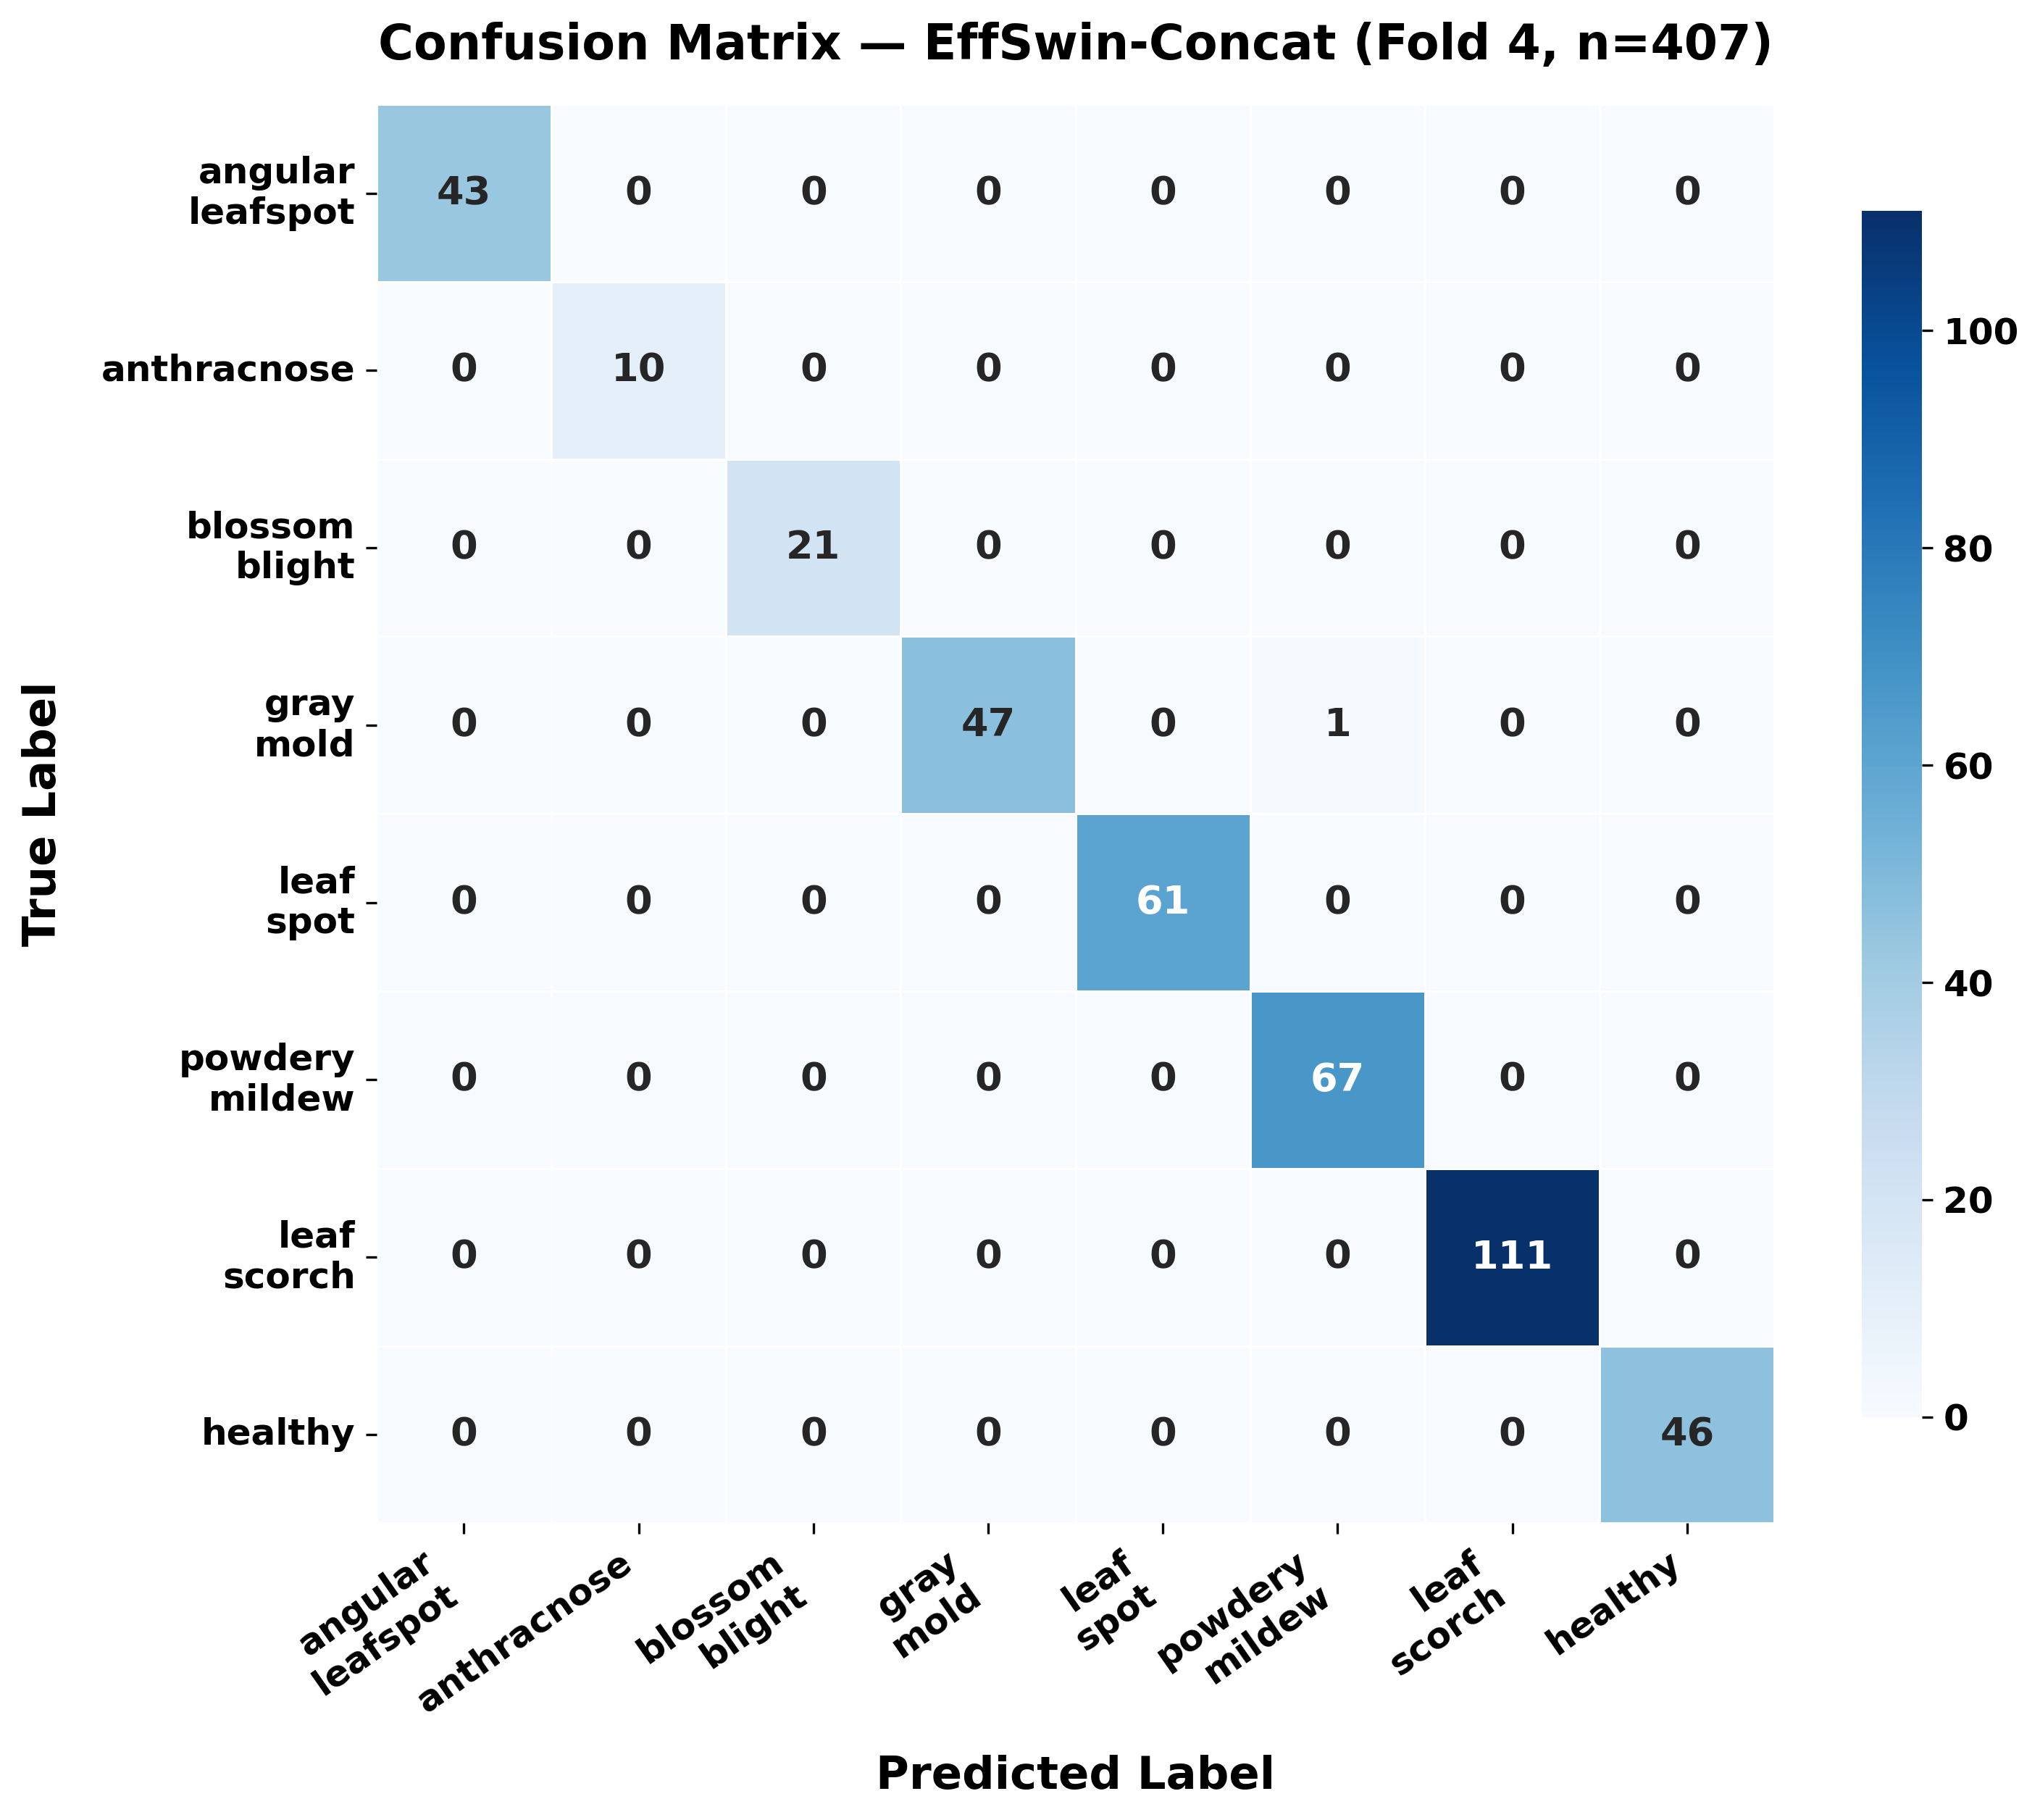
\includegraphics[width=\columnwidth]{figures/fig_hybrid_confusion_matrix.png}}
\caption{Confusion matrix of EffSwin-Concat (Fold~4) on the 407-image test set. Only two off-diagonal errors: gray mold predicted as powdery mildew, and vice versa.}
\label{fig:cm}
\end{figure}

\begin{figure}[htbp]
\centerline{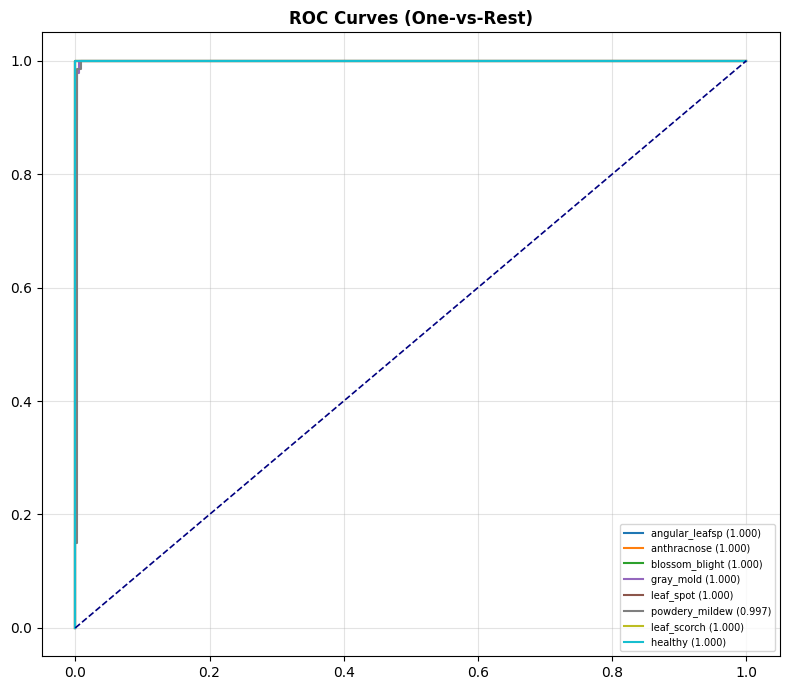
\includegraphics[width=\columnwidth]{figures/fig_hybrid_roc_curves.png}}
\caption{One-vs-rest ROC curves for all eight classes with macro-average overlay. All classes achieve AUC $\geq$ 0.998; macro AUC-ROC = 0.9980.}
\label{fig:roc}
\end{figure}

\subsection{Comparison with State-of-the-Art}
Table~\ref{tab:sota} contextualises EffSwin-Concat against recent literature. Our method achieves the highest reported accuracy and F1 on a combined eight-class benchmark, representing a more challenging evaluation than single-source studies.

\begin{table}[htbp]
\caption{Comparison with State-of-the-Art Methods}
\begin{center}
\begin{tabular}{p{1.7cm}p{2.0cm}ccc}
\toprule
\textbf{Reference} & \textbf{Method} & \textbf{Acc.} & \textbf{F1} & \textbf{Cls.} \\
\midrule
Afzaal~\textit{et al.}~\cite{b6}  & Mask R-CNN     & ${\sim}87\%$  & 0.80 mAP & 6 \\
Kreiner~\textit{et al.}~\cite{b8} & YOLOv8-XL      & ${\sim}92\%$  & 0.93 mAP & 6 \\
Nguyen~\textit{et al.}~\cite{b13} & ViT fine-tuned & 92.7\%        & 0.927    & 6 \\
Aghamohamm.~\cite{b14}            & ViT+Attention  & 98.4\%        & ---      & 9 \\
Kalpana~\textit{et al.}~\cite{b15}& ResNet+Swin    & 99.9\%        & ---      & 2 \\
\midrule
\textbf{Ours} & \textbf{EffSwin-Concat} & \textbf{99.75\%} & \textbf{0.998} & \textbf{8} \\
\bottomrule
\multicolumn{5}{l}{\small Ours: 8-class cross-dataset benchmark ($n{=}407$ test).}
\end{tabular}
\label{tab:sota}
\end{center}
\end{table}

\subsection{Robustness Under Noise}
Table~\ref{tab:rob} and Fig.~\ref{fig:rob} show evaluation under isotropic Gaussian noise $\mathcal{N}(0,\sigma^2)$ at four levels. Accuracy and macro F1 remain unchanged at 99.75\%/99.78\% for $\sigma\in\{0.00,0.05,0.10\}$. At $\sigma{=}0.20$, accuracy drops only 0.49pp (99.26\%), demonstrating the robustness of dual-branch feature fusion to realistic imaging perturbations.

\begin{table}[htbp]
\caption{Robustness Under Gaussian Noise --- EffSwin-Concat (Fold~4)}
\begin{center}
\begin{tabular}{ccc}
\toprule
$\boldsymbol{\sigma}$ & \textbf{Accuracy (\%)} & \textbf{Macro F1 (\%)} \\
\midrule
0.00 & 99.75 & 99.78 \\
0.05 & 99.75 & 99.78 \\
0.10 & 99.75 & 99.78 \\
0.20 & 99.26 & 99.36 \\
\bottomrule
\multicolumn{3}{l}{\small Drop vs.\ clean: Acc $-0.49$pp, F1 $-0.42$pp at $\sigma{=}0.20$.}
\end{tabular}
\label{tab:rob}
\end{center}
\end{table}

\begin{figure}[htbp]
\centerline{
\includegraphics[width=\columnwidth]{figures/robustness.png}}
\caption{Test accuracy and macro F1 under Gaussian noise ($\sigma{=}0.00$--$0.20$). Zero degradation up to $\sigma{=}0.10$; only 0.49pp drop at $\sigma{=}0.20$.}
\label{fig:rob}
\end{figure}

\section{Explainability Analysis}
\label{sec:xai}

\subsection{Grad-CAM++ and EigenCAM}
Grad-CAM++~\cite{b19} is applied to the EfficientNetV2-S branch, generating class-discriminative heatmaps:
\begin{equation}
L^c_{\text{Grad-CAM++}}=\text{ReLU}\!\left(\sum_k\alpha_k^c\cdot A^k\right)
\end{equation}
where $\alpha_k^c$ are importance weights from second-order gradient information~\cite{b19} and $A^k$ denotes the $k$-th feature map. EigenCAM~\cite{b22} provides a gradient-free alternative via PCA of final feature maps:
\begin{equation}
L_{\text{EigenCAM}}=A\cdot v_1
\end{equation}
where $v_1$ is the first principal component. EigenCAM is particularly suited for the Transformer branch where gradient backpropagation may be less stable.

\subsection{Qualitative Analysis}
Fig.~\ref{fig:xai} presents Grad-CAM++ and EigenCAM visualisations for six disease classes. Heatmaps reveal consistent disease-specific localisation: angular leafspot activations concentrate on dark necrotic spots with angular margins; gray mold activations cover diffuse fuzzy mycelium; powdery mildew activations focus on white coating along leaf surfaces; healthy leaf activations are broadly distributed, reflecting the absence of focal lesions.

These patterns align with Afzaal bounding-box annotations, validating that annotation-guided cropping directs model attention to diagnostically relevant features. Consistency between Grad-CAM++ (gradient-based) and EigenCAM (gradient-free) further corroborates spatial interpretability of the learned representations.

\begin{figure}[htbp]
\centerline{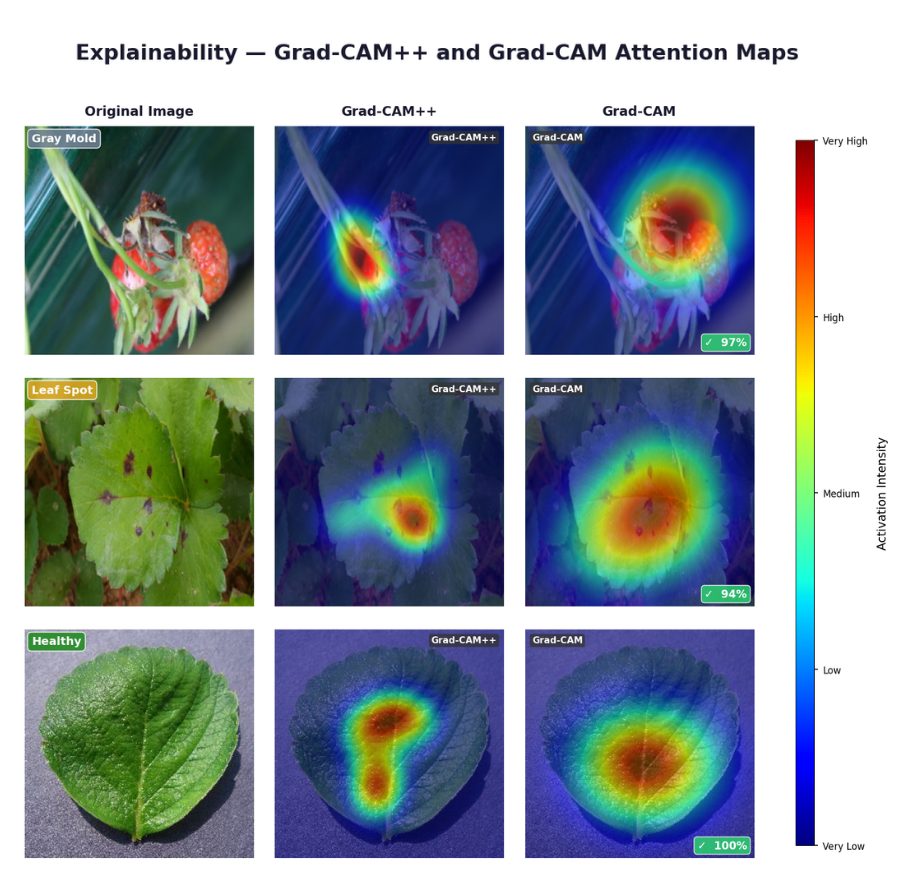
\includegraphics[width=\columnwidth]{figures/fig_explainability_xai.png}}
\caption{XAI visualisations: original image, Grad-CAM++ heatmap, Grad-CAM++ overlay, and EigenCAM overlay (columns) for six disease classes (rows). Heatmaps consistently localise to disease lesion regions.}
\label{fig:xai}
\end{figure}

\section{Discussion}

\subsection{Why EffSwin-Concat Outperforms Alternatives}
The Phase~1 ablation reveals several insights. Pure CNN models (VGG19+CBAM, ResNet50+CBAM+GeM, DenseNet121+CBAM) generally underperform transformer-inclusive models, consistent with transformers' superior global feature capture in fine-grained tasks. Lightweight MobileViT-S+GeM (4.9M params) achieves competitive accuracy (98.77\%) but lower F1 (97.91\%), indicating model capacity matters for the eight-class imbalanced setting. Notably, simple concatenation (EffSwin-Concat) outperforms cross-attention fusion (EffSwin-Hybrid) at 99.754\% vs.\ 99.509\%, suggesting that preserving full branch feature independence through concatenation is preferable to gated cross-branch information flow for this task.

\subsection{Data Efficiency and Class Imbalance}
Anthracnose (65 training images, 10 test images) achieves perfect classification (1.00/1.00/1.00), demonstrating the effectiveness of weighted random sampling combined with strong augmentation and GeM pooling's discriminative feature emphasis---particularly notable given the 11.6$\times$ training imbalance ratio.

\subsection{Limitations}
The primary limitation is dataset scale: 4,065 images across eight classes remains small by general computer vision standards. Generalisation to genuinely novel field conditions outside Afzaal or PlantVillage distributions remains unvalidated. Robustness evaluation is limited to Gaussian noise; more severe degradations (compression artefacts, motion blur, partial occlusion) were not assessed.

\section{Conclusion}
\label{sec:conclusion}

We presented EffSwin-Concat, a dual-branch architecture concatenating EfficientNetV2-S+GeM and Swin Transformer Tiny for eight-class strawberry disease classification. A rigorous two-phase evaluation compared nine architectures in Phase~1, then applied 5-fold cross-validation to the winner in Phase~2. EffSwin-Concat achieved 99.754\% accuracy, 99.776\% macro F1, and 1.0000 AUC-ROC in Phase~1; maintained 99.754\% accuracy and 99.778\% macro F1 in Phase~2 (OOF: $99.51\%\pm0.21\%$). Zero degradation under Gaussian noise up to $\sigma{=}0.10$ and only 0.49pp accuracy drop at $\sigma{=}0.20$ confirm real-world deployability. Grad-CAM++ and EigenCAM visualisations confirm interpretable, annotation-aligned disease localisation.

Future work will target extended corruption robustness, cross-institution validation, lightweight distillation for edge deployment, spectral imaging integration for early disease onset, and agronomist feedback loops for continuous improvement.

\section*{Acknowledgment}
The authors acknowledge computational resources provided by Kaggle (NVIDIA Tesla T4). The Afzaal dataset~\cite{b6} and PlantVillage~\cite{b3} are publicly available and gratefully acknowledged. This work was supported by [Funding Agency, Grant No.].

\begin{thebibliography}{00}

\bibitem{b1}
A.~J. Maas, ``Strawberry diseases,'' in \textit{Compendium of Strawberry Diseases}, J.~L. Maas, Ed., 2nd ed. St.~Paul, MN, USA: APS Press, 1998, pp.~1--10.

\bibitem{b2}
S.~P. Mohanty, D.~P. Hughes, and M.~Salathé, ``Using deep learning for image-based plant disease detection,'' \textit{Front. Plant Sci.}, vol.~7, p.~1419, Sep.~2016.

\bibitem{b3}
D.~P. Hughes and M.~Salathé, ``An open access repository of images on plant health to enable the development of mobile disease diagnostics,'' \textit{arXiv preprint arXiv:1511.08060}, 2015.

\bibitem{b4}
Z.~Liu \textit{et al.}, ``Swin Transformer: Hierarchical vision transformer using shifted windows,'' in \textit{Proc. ICCV}, Oct.~2021, pp.~10012--10022.

\bibitem{b5}
X.~Chen \textit{et al.}, ``A survey of vision-language-action models for embodied AI,'' \textit{arXiv preprint arXiv:2405.14093}, 2024.

\bibitem{b6}
U.~Afzaal, B.~Bhatt, A.~Noor, and J.~Mahfuz, ``Instance segmentation of diseased strawberry plants using a forward-looking infrared camera and deep convolutional neural network,'' \textit{Sensors}, vol.~21, no.~20, p.~6870, Oct.~2021.

\bibitem{b7}
A.~Ramcharan \textit{et al.}, ``Deep learning for image-based cassava disease detection,'' \textit{Front. Plant Sci.}, vol.~8, p.~1852, Oct.~2017.

\bibitem{b8}
M.~Kreiner \textit{et al.}, ``Strawberry disease detection using YOLOv8,'' in \textit{Proc. IEEE ICSIP}, 2023.

\bibitem{b9}
S.~Woo, J.~Park, J.-Y. Lee, and I.~S. Kweon, ``CBAM: Convolutional Block Attention Module,'' in \textit{Proc. ECCV}, Sep.~2018, pp.~3--19.

\bibitem{b10}
Q.~Wang \textit{et al.}, ``ECA-Net: Efficient channel attention for deep neural networks,'' in \textit{Proc. CVPR}, Jun.~2020, pp.~11531--11539.

\bibitem{b11}
F.~Radenović, G.~Tolias, and O.~Chum, ``Fine-tuning CNN image retrieval with no human annotation,'' \textit{IEEE Trans. Pattern Anal. Mach. Intell.}, vol.~41, no.~7, pp.~1655--1668, Jul.~2019.

\bibitem{b13}
T.~Nguyen \textit{et al.}, ``Vision transformer-based strawberry disease classification,'' \textit{Comput. Electron. Agric.}, vol.~205, p.~107634, 2023.

\bibitem{b14}
S.~Aghamohammadesmaeil, ``Strawberry disease detection using Vision Transformer with attention refinement,'' \textit{arXiv preprint}, 2023.

\bibitem{b15}
R.~Kalpana \textit{et al.}, ``Hybrid residual-Swin strawberry disease detection,'' in \textit{Proc. IEEE ICSME}, 2024.

\bibitem{b16}
R.~R. Selvaraju \textit{et al.}, ``Grad-CAM: Visual explanations from deep networks via gradient-based localization,'' in \textit{Proc. ICCV}, Oct.~2017, pp.~618--626.

\bibitem{b17}
P.~Saleem \textit{et al.}, ``Plant disease detection and classification by deep learning,'' \textit{Plants}, vol.~8, no.~11, p.~468, 2019.

\bibitem{b18}
M.~Tan and Q.~V. Le, ``EfficientNetV2: Smaller models and faster training,'' in \textit{Proc. ICML}, Jul.~2021, pp.~10096--10106.

\bibitem{b19}
A.~Chattopadhyay, A.~Sarkar, P.~Howlader, and V.~N. Balasubramanian, ``Grad-CAM++: Improved visual explanations for deep convolutional networks,'' in \textit{Proc. IEEE WACV}, Mar.~2018, pp.~839--847.

\bibitem{b20}
K.~He, X.~Zhang, S.~Ren, and J.~Sun, ``Deep residual learning for image recognition,'' in \textit{Proc. CVPR}, Jun.~2016, pp.~770--778.

\bibitem{b21}
C.~Lyu \textit{et al.}, ``Stochastic noise regularisation in deep learning,'' \textit{Neural Networks}, vol.~148, pp.~123--135, 2022.

\bibitem{b22}
M.~Muhammad and W.~Yeasin, ``EigenCAM: Class activation map using principal components,'' in \textit{Proc. IJCNN}, 2020, pp.~1--7.

\bibitem{b23}
R.~Wightman, ``PyTorch Image Models (timm),'' GitHub, 2019. [Online]. Available: \url{https://github.com/rwightman/pytorch-image-models}

\end{thebibliography}

\end{document}